\chapter{今まで通りに作る}
\section{いつも通り作ってみよう}
ヘビゲームと同じように、今までのように作ってみましょう。
\lstinputlisting[title={今までのような作り方}, language=Python]{chapter2/tetris.py}
\newpage
\subsubsection{実行結果}
ここまでできたら、次の章に進んでください。実行結果も載せてあるので比べてみてください。
\begin{figure}[h]
  \centering
  % 824x1600
  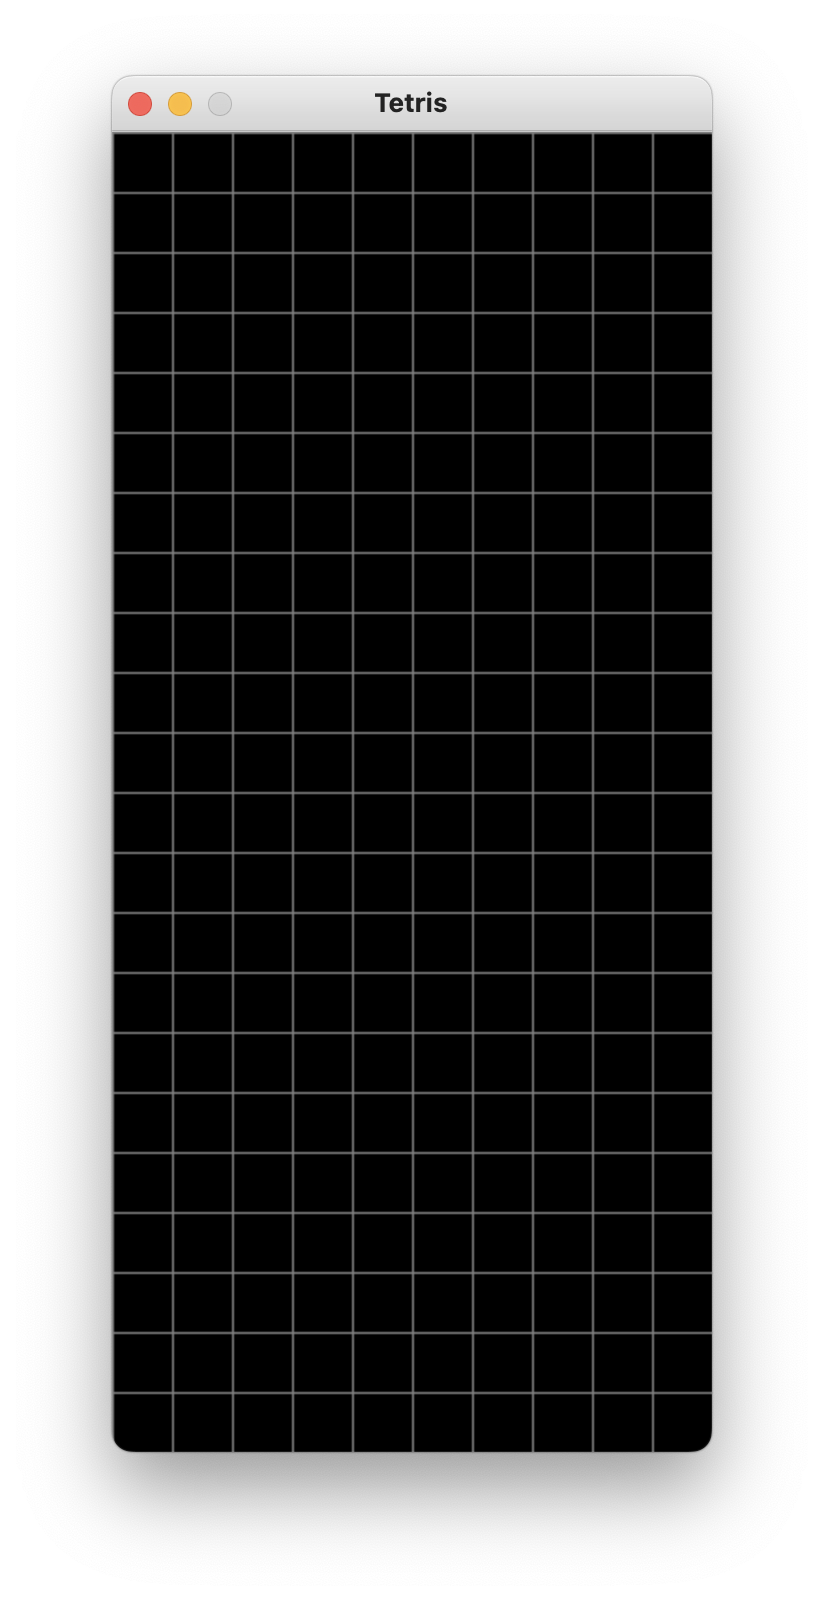
\includegraphics[height=15cm, natwidth=824,natheight=1600]{images/TetrisCH1_1.png}
  \caption{テトリスの実行結果}
\end{figure}